\documentclass[../main.tex]{subfiles}
\begin{document}

\chapter{Methods}
\labch{methods}

\section{GWAS}

In this section I shall describe some well established methods which 
were applied in some of the papers described in the thesis.

\section{Regression}
\labsec{regression}

Regression usually consists of three-steps:

\begin{enumerate}
	\item Assumption making, where one chooses the parameters of the 
		model and stuff.
	\item Fitting of the model on a training dataset.
	\item Prediction on a testing dataset.
\end{enumerate}

\newthought{Linear regression\cite{James2013}} is used to model a linear 
relationship between a continuous variable, $Y$, and one or more other 
variables, the $X$'s, which may be continuous or categorical. In other 
words, $Y$ can be expressed as

\begin{equation}
	Y \approx \beta_0 + \beta_1X_1 + \beta_2X_2 + \ldots + \beta_pX_p\,,
\end{equation}

where the $\beta$'s are called the model coefficients; the approximation 
sign is due to random errors, which causes the $Y$ to differ from the 
right-hand side by a term $\epsilon$ --a random error. The purpose of 
simple linear regression is first to fit the model, \ie to find the 
values of the coefficients that better describe the relationship between 
$X$ and $Y$ in a training dataset, and then to apply the model to make 
predictions of $Y$ on a testing dataset with known $X's$. The fitted 
model, where the parameters are estimated, is usually represented as 
follows:

\begin{equation}
	\hat{y} = \hat{\beta}_0 + \sum_{j=1}^{p}\hat{\beta}_j x_j\,.
\end{equation}

The estimation of the coefficients is often made by the minimisation of 
the residual sum of squares, which is defined as 
$\sum_{i=1}^{n}(y_i~-~\hat{y_i})^2$, \textit{i.e.}\ 
$\sum_{i=1}^{n}(y_i~-~(\hat{\beta}_0~+~\sum_{j=1}^{p}\hat{\beta}_jx_j))^2$.

The coefficients are obtained by using some calculus to find the partial 
derivatives of the RSS function with respect to all the $\hat{\beta}$, 
and then some algebra to solve a $p$th-order linear system where we 
impose such derivatives equal to $0$.
\marginnote{When $p=2$, the partial derivatives are
\begin{flalign*}
&\frac{\partial RSS}{\partial \hat{\beta}_0} =
	\sum_{i=1}^{n} -2 (y_i - \hat{\beta}_1 x_i - \hat{\beta}_0)
&\\
&\frac{\partial RSS}{\partial \hat{\beta}_1} =
	\sum_{i=1}^{n} -2 x_i (y_i - \hat{\beta}_1 x_i - \hat{\beta}_0)
\end{flalign*}
and the system yields
\begin{flalign*}
&\hat{\beta}_0 = \bar{y} - \hat{\beta}_1\bar{x}
&\\
&\hat{\beta}_1 = \frac{\sum_{i=1}^{n}(x_i - \bar{x})(y_i - \bar{y})}
	{\sum_{i=1}^{n}(x_i - \bar{x})^2}
\end{flalign*}
}

Once we have the coefficients, given an $x$, we could estimate an 
$\hat{y}$; geometrically, $\hat{\beta}_0$ is the $y$-intercept of the 
regression line and $\hat{\beta}_1$ is its slope.

\newthought{Ridge regression\cite{James2013}} is a regularisation method 
which allows to reduce the dependance of the fitting on the training set 
of values by shrinking the coefficients towards zero. This is achieved 
with a slight modification of the least squares, that is, the function 
to minimise is

\begin{equation}
	\sum_{i=1}^{n}\left(y_i-\beta_0-\sum_{j=1}^{p}\beta_jx_{ij}\right)^2+
		\lambda\sum_{j=1}^{p}\beta_j^2\,.
\end{equation}

This function is the sum of the RSS and a penalty term, the minimisation 
of which can improve the fitting of the model, provided that the tuning 
parameter $\lambda$ is properly chosen.

\newthought{Lasso regression\cite{Tibshirani1996}} is another 
regularisation method which allows to effectively select a subset of 
relevant predictors by setting the coefficients of the others to zero. 
In this case, the minimisation function is

\begin{equation}
	\sum_{i=1}^{n}\left(y_i-\beta_0-\sum_{j=1}^{p}\beta_jx_{ij}\right)^2+
		\lambda\sum_{j=1}^{p}\left|\beta_j\right|\,.
\end{equation}

\newthought{Elastic net regression\cite{Zou2005}} combines the best 
features of ridge and lasso regression by introducing two penalty terms:

\begin{equation}
	\sum_{i=1}^{n}\left(y_i-\beta_0-\sum_{j=1}^{p}\beta_jx_{ij}\right)^2+
		\alpha\sum_{j=1}^{p}\left(\beta_j\right)^2+
		(1-\alpha)\sum_{j=1}^{p}\left|\beta_j\right|\,,
\end{equation}

with $\alpha$ between 0 and 1. Its main advantage is that it works well 
when $p>n$, for it can potentially group correlated predictors and 
select only one representative variable for each group.

\newthought{Logistic regression\cite{James2013}}, which applies when the 
predicted outcome is a binary variable indicating whether the response 
falls into one of two categories, models the probability that the 
variable belongs to a particular category.

While for linear regression we assumed an equation of the form of a 
straight line (or a multi-dimensional equivalent), for logistic 
regression we need a function that returns values between 0 and 1, thus 
we rely on the logistic function

\begin{equation}
	Y = P(Z = 1 | X) =
		\frac{\exp(\beta_0+\beta_1X)}{1+\exp(\beta_0+\beta_1X)}\,.
\end{equation}

\begin{marginfigure}[0cm]
	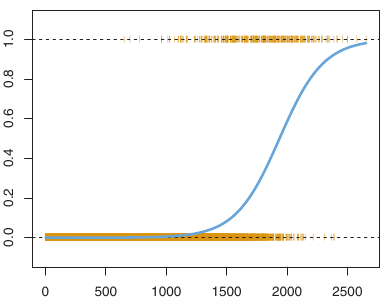
\includegraphics{methods/logistic}
	\labfig{logistic}
	\caption{An example of logistic model. Adapted from James etal 2013, 
		"An introduction to statistical learning".}
\end{marginfigure}

In order to fit this model we switch to the \enquote{estimated} values, 
denoted by an hat, and manipulate the logistic function until we have

\begin{equation}
	\log\left(\frac{\hat{y}}{1-\hat{y}}\right) =
		\hat{\beta}_0 + \hat{\beta}_1 x\,,
\end{equation}

where the left-hand member is the logarithm of the odds, or logit. At 
this point the coefficients can be found with the maximum likelihood, 
and the predictions be made. As with linear regression, this model can 
be easily extended to include more than one predictor.

\end{document}
